\RequirePackage{ifpdf}
\documentclass[11pt, final]{ucthesis}
% Look at the README first!  It's short!

%%% \documentclass[11pt/12pt/10pt, final/draft/comment]{ucthesis}
%%% The first argument is the text size. The second argument changes
%%% The margins and the spacing.
%%% FINAL mode prints double spaced with figures and thesis margins.
%%% DRAFT mode prints single-spaced with 1" margins, with slightly
%%%   narrower margins for the figure captions so that they stand out.
%%% COMMENT mode prints an extra wide right margin and tiny margins
%%% everywhere else. This allows your committee plenty of room to add
%%% comments.
%%% Margins can be changed in the last lines of the ucthesis.cls
%%% with the geometry command.

% This information will get stored inside the PDF file
%\pdfinfo{
%       /Title      (U. C. Berkeley Dissertation)
%       /Author     (Your Name Here)
%       /Keywords   ()
%    }

% This gives you control over how far down in the hierarchy the
% table of contents will print. I use 2.
\setcounter{tocdepth}{2}

% This allows me to add directories to the graphics path
% so that I don't need to specify directories in the individual
% LATEX paths.
% EACH PATH MUST END IN A '/'
% In other words, \includegraphics{Fig1} will first look in the current
% directory, but if it can't find the file Fig1, it will  look for
% SUBDIRECTORY/Fig1 . If that's not there, it will look next in
% SUBDIRECTORY2/Fig1 . If it finds that, it will ignore anything after
% SUBDIRECTORY2.
%
% As I have them now, they are:
\graphicspath{{introduction_figs/},{MORE_figs/},{EVENMORE_figs/}}

% ========================================= Extra commands
% Degree Symbol
\newcommand\degrees{\ensuremath{^\circ}}
\newcommand{\tab}{\hspace{5mm}}
\newcommand{\blankpage}{\clearpage ~ \newpage}


% ========================================= DOCUMENT
\begin{document}

% Declarations for Front Matter

% TITLE
\title{BeaverDam: Video Annotation Tool for Computer Vision Training Labels}

% NAME
% Note that this must be exactly as it appears in University records.
\author{Anting Shen}

% PREVIOUS DEGREES
% Put each previous degree on its own line in the following format:
\prevdegrees{}

% DATE OF GRADUATION
% This text will appear on the title page
% Note that degrees are only granted in Fall and Spring at Berkeley.
\degreemonth{Fall} \degreeyear{2016} \degree{Master of Science}
% This text will appear on the abstract page.
% For Berkeley, it should be identical to the graduation month.
\defensemonth{Fall} \defenseyear{2016}

% COMMITTEE MEMBERS
% You can have up to 5 members listed separately.
%After that, you throw them all into the "other members" category.
\numberofmembers{2}
    \chair{Professor Kurt Keutzer}
    \othermemberA{Professor Trevor Darrell}

% DEPARTMENT/DEGREE PROGRAM
%Your Department. Make sure this is the department and/or program
% name that you are enrolled in...
\field{Computer Science}

% CAMPUS NAME
% Your UC Campus, e.g., "Berkeley"
% Note that if you are not at Berkeley, you may have to modify the
% ucthesis.cls to change the wording on the Title page.
\campus{Berkeley}


\begin{frontmatter}

% ===============================================
% MAKE THE TITLE PAGE
% ===============================================
\maketitle


% ===============================================
% APPROVAL SIGNATURE PAGE
% ===============================================
\approvalpage

% ===============================================
% Copyright Page
%
% The copyright page is optional. However, the University
% thesis guide says that a blank page should be inserted
% if no copyright information is included.
% ===============================================
% \copyrightpage
% or the blankpage
% \blankpage

% ===============================================
% ABSTRACT
%
%   The Abstract should be stored in a file called abstract.tex
%   "It is preferred that the abstract text be less than 350 words"
%   Also generates a signature line at the end of the abstract
% ===============================================

 \abstract
    We present our annotation tool for frame-by-frame video bounding box annotation.
The framework has been used in conjunction with Amazon Mechanical Turk as well as standalone, to annotate datasets for Berkeley Deep Drive and BMW.
To accomplish this, we built upon ideas from previous works in this area, and we present our improvements and optimizations upon their user interfaces.
We also introduce the idea of tuning such an annotation tool to reduce researcher's friction, which we argue is just as important as improving workers' workflow due to the high cost of researcher time.
We share our experiences with existing tools, and our ideas (and code) for how to make the experience better for researchers.
We hope our findings and contributions further reduce the cost of producing a labeled video dataset, and introduce ideas that will improve the quality of such software in the future.

    \abstractsignature  % This prints a signature line for the chair to sign.
\endabstract

\end{frontmatter}

% ===============================================
% OPTIONAL MATERIAL
% Everything after this is optional and can appear in any order
% you desire.
\begin{optionalFrontMatter}

% ===============================================
% TABLE OF CONTENTS
% \addcontentsline{toc}{chapter}{Contents}        % Put the table of contents in the table of contents
\tableofcontents

% COMMENT OUT THIS LINE IF YOU WANT TITLE HEADERS
% THROUGHOUT YOUR DOCUMENT
\pagestyle{plain}

% Insert the List of Figures and List of Tables after the TOC
% Like everything in this section, these are both optional.
% \listoffigures
% \listoftables

% \begin{acknowledgements}
% \addcontentsline{toc}{chapter}{Acknowledgements}
% % The Acknowledgements section should be stored in a file called acknowledgments.tex
%     Thanks to Professor Keutzer and everyone in our group for the motivation and advice, Kosta for the great support, and Bichen Wu \& Byung Gon Song for sharing in the struggles.

I'd also like to acknowledge Allen Wang, Sean Zhu, and Gabriel Arreola for contributing code to this project, coming up with awesome logos, and puns.

Lastly, thanks to all the turkers who helped annotate videos, especially David Tarr, Connor Munsinger, Allen Chov, and Aljosa Cucak for their feedback.

% \end{acknowledgements}

% \begin{vitae}
% %% The Vitae section should be stored in a file called vitae.tex
%     
\begin{vitaesection}{Education}
\item [1992] University of South Babylon

B.S., Geological and Environmental Sciences

\item [2001] Diploma Factory State College

M.S., Geology

\item [2004] University of California Berkeley

Ph.D., Geology
\end{vitaesection}


\begin{vitaesection}{Personal}
\item [Born] April 18, 1906, 
San Francisco, California
\end{vitaesection}

%\begin{vitaesection}{Biographical Sketch}
%\item [] 
This can either be a formal CV, or include a more narrative biographical sketch. This is where people who discover your thesis decades down the road will find out about who you were.

%\end{vitaesection}


% \end{vitae}

% BLANK PAGE AFTER VITAE
\blankpage

\end{optionalFrontMatter}
%%%% END FRONT MATTER...


% ============================= DISSERTATION TEXT
% Begins regular arabic numeral page numbers...

\begin{dissertationText}
\renewcommand{\baselinestretch}{1.66}

% CHAPTERS
\chapter{Introduction
    \label{chap:introduction}}    % Put the title of the first chapter on this line
    Deep learning applications in recent years have come to require rapidly growing amounts of labeled training data.
Often, accuracies can be boosted by adding data as much as by spending years on algorithmic development.
For example, on the VOC07 benchmark, Faster-RCNN~\cite{FasterRCNN} with VGG-16 was able to eliminate 27.5\% of errors in the much older R-CNN~\cite{RCNN} backed by an equally old neural network architecture (mAP improved from 58.5 to 69.9). 
However, simply by including additional data from VOC12 and COCO, 29.5\% of the remaining error was eliminated (mAP improved from 69.9 to 78.8). 

\begin{figure}[h]
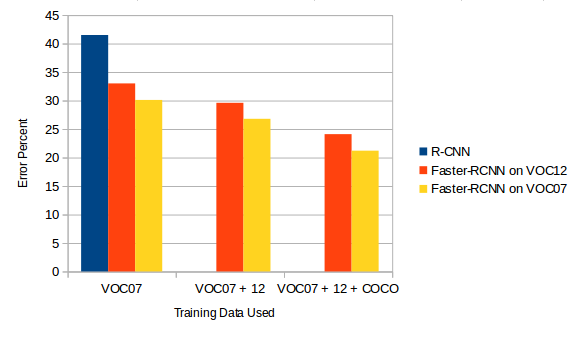
\includegraphics[width=14cm]{figs/data_vs_error.png}
\centering
\caption{Improvement of error as data increases, compared to error improvements due to algorithm improvements. 
As we can see by comparing the drop from RCNN to Faster-RCNN on VOC07 only, and the drop from adding training data to Faster-RCNN, increasing data contributes significantly to error reduction.}
\end{figure}

Therefore, for real-world application development, data can be cheaper and more effective than scientists. 
While many existing tools support image classification -- it is even built into Amazon Mechanical Turk (MTurk) -- and some tools support bounding box labeling in images, few tools exist for frame-by-frame labeling in videos. 
VATIC~\cite{Vatic} stands out as being one of the best, as not only does it make high quality annotations one of its main goals, but also cost and scalability. 

My work borrows and improves upon many concepts and results from VATIC's user studies, but I focus on an additional goal that is extremely important in creating datasets for real applications. That goal is researcher happiness.
Although VATIC extensively tested its ``User Interfaces'', I argue in chapter~\ref{chap:experimenter} that both the annotators and the experimenters are users, and the interfaces should be smooth for both when creating a tool.

Then, in chapter~\ref{chap:annotator}, I discuss my take on VATIC's User Interface principles for the annotator, and improvements upon them.

I also release all related code for BeaverDam, my video labeling platform, on Github.\footnote{http://github.com/antingshen/beaverdam}

\section*{Related Work}
\label{sec:related}

Static image annotators

Youtube video dataset

Vatic, LabelMe, etc

Things other people cite

KITTI, Berkeley group, samasource
  %% Adds the contents of the file introduction.tex
    %%% The file should have no preamble -- the chapter body.

\chapter{Experimenter Interface
    \label{chap:experimenter}}
    
During our investigation, we had many frustrating experiences with existing research tools in this area.
These included installation issues, configuration issues, and dealing with unintuitive and undocumented interfaces.
For example, there are dozens of open issues without solutions on the VATIC GitHub,
and its installation script fails at multiple points on a brand new Ubuntu box.
Due to preciousness of researcher's time,
we believe the ability for researchers to test and iterate quickly is just as important as worker speeds when it comes to video annotation.
Therefore we have placed improving the experimenter's experience as one of the main goals of this work.

\section{Interface for researcher}

For a basic user creating a crowdsourced video dataset using the default configurations we used,
BeaverDam provides a streamlined interface.
We provide a setup script that is tested on clean installs of Ubuntu 14.04 and Ubuntu 16.04.
In comparison, VATIC was tested on an unspecified Ubuntu installation with exact Apache and MySQL installs,
and while the install script claims that it should work on any operating system in theory,
installation is difficult in reality.
Additionally, our install script configures everything from Nginx and TLS to database config and backups.
The user only needs to place their credentials in the locations specified in our documentation.
While a containerization system such as Docker would have also solved VATIC's issues and ensure future compatibility,
we felt that the additional complexity is not worth it, as many of our users in the research community are unfamiliar with Docker.

To use BeaverDam after installation, we provide a web interface for researchers to easily add and view videos and jobs.
We feel that this is superior to VATIC's command line based approach,
as the number of flags needed to specify various configurations was overwhelming.
However, to allow experimenters to load large number of videos or perform other tasks programmatically,
BeaverDam also provides a Python shell interface, backed by Django, to expose every functionality through Python.

Lastly, as BeaverDam is HTML5 video based, no frame extraction step is necessary.
H.264 encoded videos will work without preprocessing.
However, we do provide scripts to convert these videos to images with matching annotations to feed into machine learning tools if desired.

\section{Decoupled modules}

As the users of BeaverDam will most likely need to modify BeaverDam to fit their needs,
we've emphasized modularity in our designs.
Since modularity is something VATIC did well with their turkic, vatic, and pyvision splits,
we've taken a similar approach.
Our infrastructure is split between a crowdsourcing module, an annotation module, and a CV-based tracking module.
But we decided to go a step further and make other parts of our platform replaceable as well.

To serve videos, we've provided Nginx to allow VATIC users to continue serving videos efficiently on the same server as their application.
But to allow for scalability, users can use AWS S3 or any other CDN, or even a mix, by specifying so when creating jobs.
Similarly, our setup pipeline is done through Ansible, a configuration management tool popular in industry.
This allows users to deploy on their own servers, or in the cloud.

We also understand that not everyone wants to use Amazon Mechanical Turk.
While past research has proven Mturk to be efficient and reliable,
companies in industry seeking training data may prefer alternatives such as CrowdFlower,
or may even choose to label in-house, or outsource to contractors.
BeaverDam is designed with this flexibility in mind as it carries its own authentication and works independently of Mturk.
This allows companies with the resources to seek cheaper labor in other countries to use BeaverDam as a platform for their workers
and track progress and pay without the need for Amazon Mechanical Turk, which carries a 20\% fee.

\begin{figure}[h]
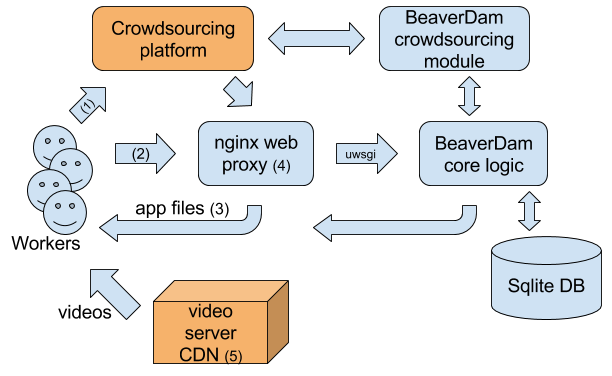
\includegraphics[width=14cm]{figs/backend.png}
\centering
\caption{BeaverDam's backend server logic. The annotation app is sent in (3). Workers can either be hired through a crowdsourcing platform (1), or hired in-house and use BeaverDam directly (2). The web proxy (4) smoothly handles many requests and forwards static files, and performs HTTPS authentication with HSTS to meet Mturk security requirements. A video server or cloud provider CDN (5) is used to reduce worker download waiting times, a problem of other video labeling tools.}
\end{figure}

\section{Patterns}

To facilitate modification of our code, we adopted the Django framework because it sets fairly strict conventions on how a project is structured.
Someone familiar with Django will immediate know where to find the files responsible for each function of the backend.
As there is a fair bit of frontend logic to video annotation, we've organized the code responsible according to well defined patterns as well.
Under Our Pattern Language ~\cite{opl}, the frontend follows the Model-View-Controller structure, and each of the three components is event-based.
While using events to communicate within an application may seem like additional complexity at first, it enables decoupling and extends the existing events from user interaction.

\section{Dependencies}

The number one problem we encountered during our installations of VATIC was broken dependencies.
Its GitHub issues point to problems users are having due to MySQL, cython, ipinfodb, and gcc versioning.
BeaverDam addresses this problem in two ways.
First, we greatly reduce the number of dependencies.
Python 3 and two python packages installed through pip are the only dependencies required to run BeaverDam.
Three other dependencies, Nginx, supervisor, and uwsgi, are recommended for efficient deployment.
And to avoid the burdensome installation and configuration of a database that VATIC required, we use sqlite3, which is a Python standard library.
In this case, it proves to be enough to handle even a fairly large amount of annotations, and can be swapped out easily if needed.
Second, we version each dependency.
This ensures that newer versions of dependencies in the future cannot break compatibility.
For front-end libraries, we check-in the required files directly instead of using a package manager, avoiding extra complexity.

Another problem we encountered with VATIC's dependencies was its system-wide installation and configurations.
Different users sharing a server would often leave bad state for others, causing hard-to-track bugs.
We enclose the project in a virtual environment, and we include an idempotent script that verifies all required state, and fixing them if necessary.
Our system is designed to be quickly set up on new VM instances,
so one can perform upgrades and fixes by discarding the entire server VM and starting from scratch.

When choosing our dependencies, we strived to use the latest versions of mature technologies.
We use Python 3.5 and Django 1.10, the latest versions available at the time.
We also use the ES6 version of JavaScript, which includes many features to enhance readability and programmer happiness.
While alternatives such as TypeScript provides additional features, ES6 is supported without a transpiler and avoids complexity.
Browser compatibility of ES6 was a small issue with workers, but we expect this to improve as browsers fully adopt the standard and workers update to the latest version of their browsers.

\section{Security}

As BeaverDam aims to be industry quality software instead of research quality, security considerations are important.
While one would not expect malicious users, it's important to follow security best practices as a preventative measure.
Furthermore, having a full set of security tools allows the app to perform its own authentication,
adding to modularity by allowing it to function as a standalone app without Mechanical Turk, unlike VATIC.

The first and best line of defense is regular backups.
To back up data and configuration in VATIC, one had to perform a MySQL database dump and ensure all config files around the server are duplicated.
In BeaverDam, configuration is checked into version control, and the database is in a single file for easy backup and restore thanks to Sqlite.
Our setup tool automatically sets a daily backup to Amazon S3 if the app is configured with access keys.
We also implemented other critical security features, such as TLS, HSTS, CSRF protection, and clickjacking protection.
These features are automatically installed and activated by our setup script,
with the user only needing to provide TLS certificates for their domain. \footnote{We recommend \textbf{letsencrypt} for easy and free TLS certificates.}



\chapter{Annotator Interface
    \label{chap:annotator}}
    \begin{figure}[h]
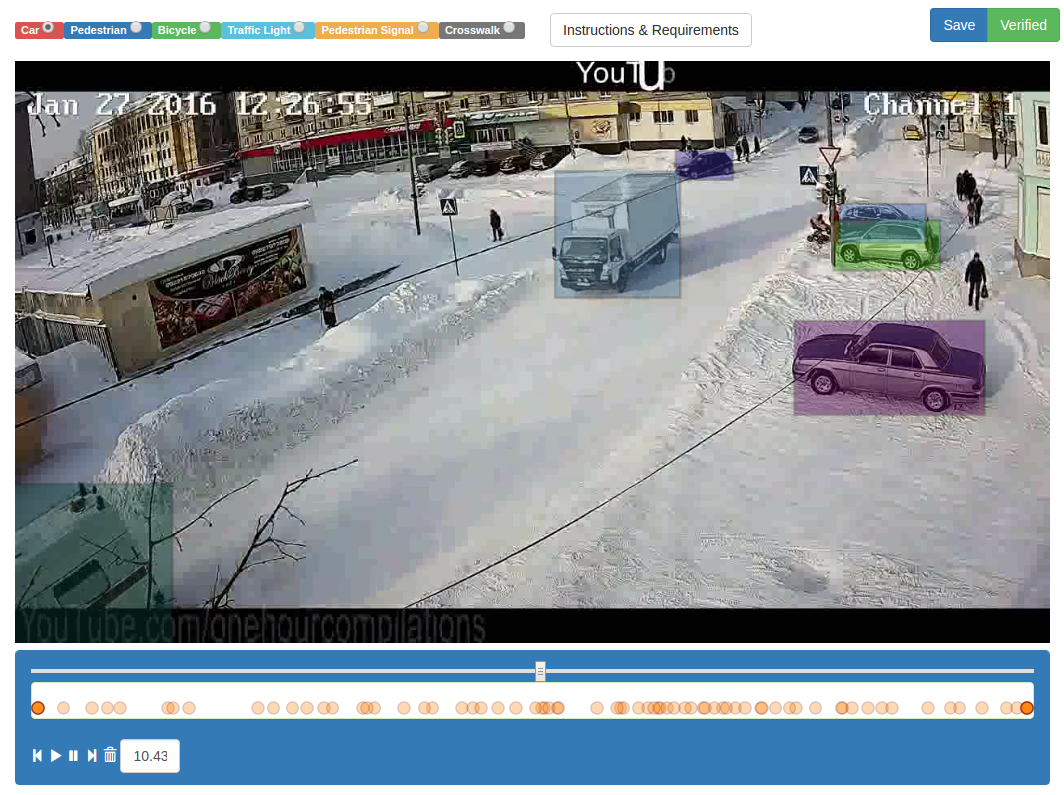
\includegraphics[width=15cm]{figs/interface.png}
\label{interface}
\centering
\caption{BeaverDam's expert verification interface with user keyframe scheduling enabled, border buffer disabled. Workers see a similar interface. Note the keyframe scheduling interface integrated with the video player, the single click multiple create interface, and objects being allowed to move partially or wholly off-screen in the bottom left corner.}
\end{figure}

The productivity of annotators is the focus of most of the prior works in this area.
During the development and deployment of BeaverDam, we've gathered extensive feedback from our turkers and testers.
We also implemented features suggested by past works such as VATIC,
and introduced several new ones to address issues found during the testing of VATIC.\footnote{Sceenshots of select issues in this chapter are taken from the demo video on VATIC's website, and are representative of what we encountered.}


\section{Keyframe scheduling}

A big decision for a keyframe-based video annotation tool is whether the worker or the tool chooses the keyframe schedule.
From past user studies, we know that human workers don't always choose the best keyframes, leading to inefficiencies.
In fact, VATIC showed that by switching to a fixed keyframe schedule, workers were able to label faster.
However, in our studies we found it to not always be the case.
Since our videos contain a varied mix of stationary objects, slow \& linearly moving objects, and fast objects with irregular motion, it makes sense to use fewer keyframes for easier objects.
While a flexible keyframe schedule could potentially be automated using tracking, we instead optimized the interface for user created keyframes.

We added a keyframe viewer bar that displays all keyframes and keyframes for the currently selected object.
The user can click on these keyframes to edit them, or insert new keyframes by editing the boxes when on a frame that's not a keyframe.
We also included keyboard shortcuts to jump between keyframes for experts who need fine-grained editing.

\section{Video playback for maintaining identity}

VATIC's video player was a rudimentary image changer as its purpose was to give workers context when tracking objects.
As we wanted more flexibility and power for more advanced labelers, we incorporated a full fledged video player over VATIC's usage of JavaScript to advance images of frames.

One huge issue we solved with this setup was video loading times.
When deploying VATIC, we found users complaining about load times, and sometimes jobs would time out before the video loaded, especially when using high resolution images for frames.
When seeking in the video, the images would flash to white if it's not loaded from cache quickly enough.
The interruption caused not only context loss but also frustration.
By converting the app to use HTML5 video, we take advantage of the ability to stream, similar to how YouTube and other sites can display the video without loading all of it first.
The annotator can then begin annotating as the video loads.
The playback is also much smoother, with a minor tradeoff of slightly slower rewinds, as videos are encoded in a way optimized for forward playback.
This was an improvement overall as workers used forward playback more often than rewinds.

\section{Reducing clicks}

In addition to measuring the time it takes for annotators to perform certain actions, we sought to minimize the number of clicks necessary.
We find this to be a good rule of thumb when we don't have enough users to properly A/B test design choices.

First, we set the user in the hybrid create/edit mode by default.
A new object is created if the user drags in an empty spot, and an existing object is edited otherwise.
VATIC requires the user to click a ``create'' button, which enables the user to annotate heavily overlapped objects more easily.
We propose that it's more efficient to force a user to perform the extra steps of creating a box in an empty spot and dragging it onto the object in case of overlap,
as heavy overlaps turned out to be rare in our datasets, so it was better to optimize for the common case.

\begin{figure}[h]
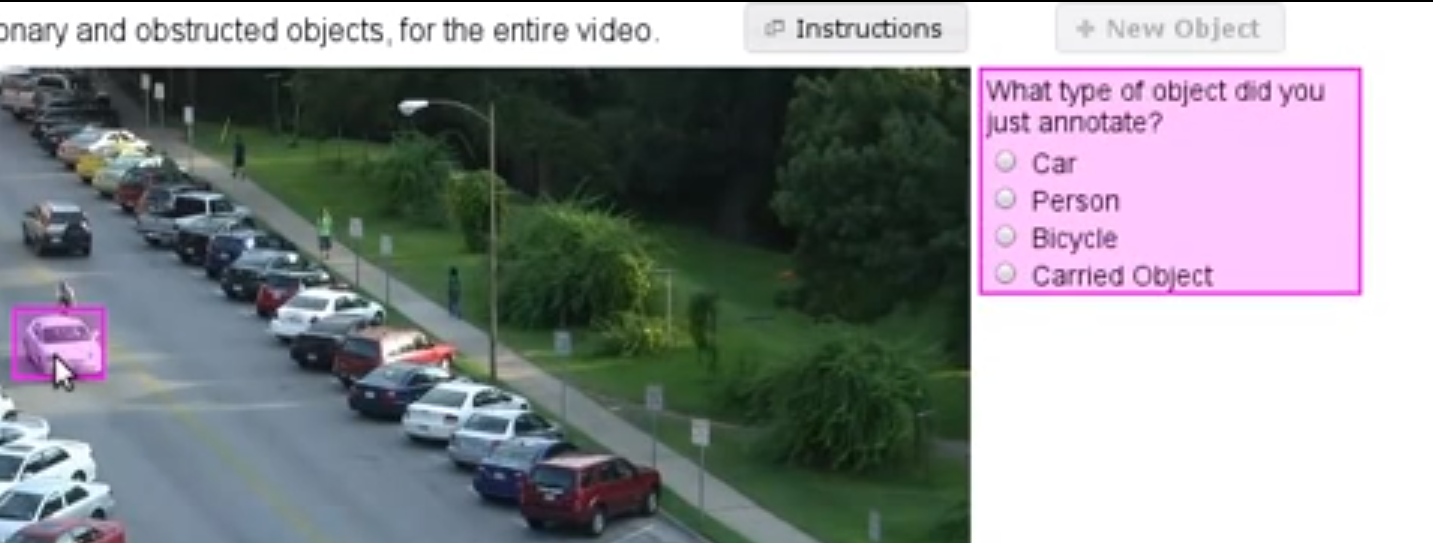
\includegraphics[width=14cm]{figs/vatic_create.png}
\centering
\caption{Explicit object creation in VATIC. BeaverDam guesses whether the worker wants to create a new object or edit an existing one by where they click, which is efficient in the general case. We also eliminate this additional prompt of asking for the object type and assume the type is same as the last created type by default.}
\end{figure}

Additionally, instead of having the user choose the type of object each time, we default to the most common label (car) or the user's last selection.
This reduced clicks, but did result in more errors for new users who didn't notice that they must change the label from the default when labeling non-cars.
While VATIC's prompting each time prevented this, we elected to solve it through a better tutorial to save time for acclimated annotators.

Finally, BeaverDam includes extensive keyboard shortcuts, with the aim of eliminating any need for the mouse aside from drawing and moving boxes.
Tasks such as label selections and video playback are all controlled through the keyboard.
We left in optional mouse controls, but it may be a good choice to remove them to enforce the faster keyboard workflow.
Surprisingly, we have had turkers report that they were on tablets, and keyboard shortcuts were inefficient for them.
However, we find in our small sample of annotators that tablet users are few, and less efficient in general.

\section{Handling frame exit/enters}

During our user tests, we found that users have the most difficulty when objects are entering or exiting the frame, as it's difficult for linear interpolation to handle a box whose size is increasing but one edge is fixed to the edge of the frame.

\begin{figure}[h]
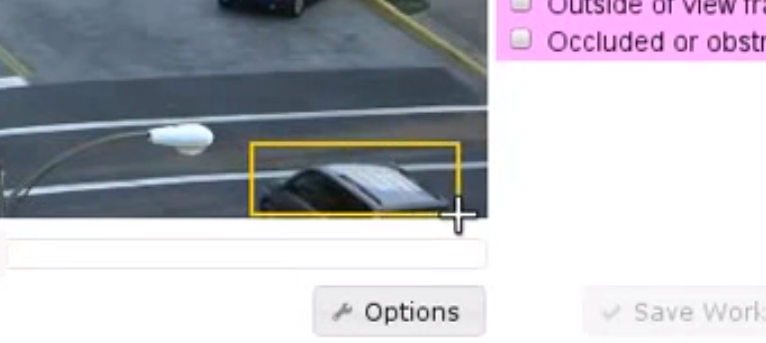
\includegraphics[width=14cm]{figs/vatic_border.png}
\centering
\caption{VATIC annotation of object entering frame. Note the user must draw the box exactly to the edge of the screen as shown here, as drawing fails otherwise. BeaverDam allows the user's mouse to draw to outside the frame, cropping back to the frame edge in post processing.}
\end{figure}

This was one of the main challenges when annotating using VATIC, as we had many driving videos where objects frequently entered and exited.
To address this issue, we introduced two solutions.
First, we allow boxes to be partially or wholly located outside the frame.
This enables the user to guess at the true location of the object if the frame were bigger, which allows for much better linear interpolation. % TODO: EXAMPLE OF THIS
Then, we add a large padding around the border of the frame, essentially enlarging the frame with blank space, which makes drawing and editing boxes that are located partially outside the frame much easier.
After labeling, any boxes that are partially outside the frame can be cropped to the edge of the frame.


% \section{Micro vs Macro tasks}

% The topic of whether to divide up work to give each worker a small task to be completed in less than a minute (micro task) has been well discussed in literature.
% In ImageNet and other image classification \& detection datasets, micro tasks were preferred as they provided the workers more predictable task completion times and reward schedules.
% They are also easier for quality control as gold standard tasks where the label in known can be dispersed among the tasks.
% However, the authors of VATIC found through their experiments that macro tasks were better for video annotation, as errors from earlier tasks propagated throughout the rest of the video.
% We compared these two competing philosophies of expert annotators completing large tasks vs using many independent small tasks.



% Comparison from existing literature

% Proposal advocating for micro-tasks in video labeling

% Extensible task structure

% \section{Interpolation \& Tracking}


\chapter{Conclusion
    \label{chap:conclusion}}
    We have presented numerous improvements to existing video annotation tools.
We first argued that optimizing for researcher time is as important, if not more important than optimizing for worker efficiency, and showed our contributions in that area.
Then we demonstrated several ideas that allow for easier annotation by the workers that we discovered in our experiments.
We showed how BeaverDam enables cheaper annotations to create large datasets that improve model accuracies in production.

As BeaverDam is designed to be extensible, we hope that the platform will adapt to new types of annotations.
BeaverDam's modular designs shine best when new types of data, such as point clouds from LIDAR, require human labeling in the future.





% Start Bibliography on its own page
\clearpage

% This was the most significant change I made to the original style file.
% The template now accepts the IEEE-style .bib files that I was already using
% for my papers.  -Niels Hoven 5/24/2005
% You can substitute the name of another bibliography style file here.
\bibliographystyle{IEEEtran}
\addcontentsline{toc}{chapter}{Bibliography}
\ssp    % SINGLE SPACE REFERENCES (optional)

\bibliography{IEEEfull,thesis}


% ------------------- OPTIONAL APPENDICES
% \appendix
% \chapter{Allocated spectrum for communications
%     \label{appen:commspec}}
%    
source: Comsearch~\cite{Comsearch}

\begin{table}[htp]
 \begin{center}\begin{tabular}[t]{|c|c|}
 \hline
Category &  Allocation \\
\hline

Microwave & 609 MHz  \\
\hline

Broadcast & 423 MHz\\
\hline

Satellite & 188 MHz  \\
\hline

Point-to-Multipoint & 203 MHz  \\
\hline

PCS/Cellular & 193 MHz   \\
\hline

ISM & 110 MHz    \\
\hline

Other & 1274 MHz   \\
\hline

\end{tabular}
\end{center}
  \caption{\footnotesize{Spectrum under 3 GHz}
   \label{table:categories}}
\end{table}

\end{dissertationText}
\end{document}

% Congratulations, Doc!
